\newpage
\section{Time domain editor}
Related YouTube videos:
\begin{figure}[H]

\begin{tabular}{ c l }


\includegraphics[width=0.05\textwidth]{./images/youtube.png}

&
\href{https://www.youtube.com/watch?v=D7yJLFmTAVQ}{Simulating optoelectronic sensors made from polymers.}

\end{tabular}
\end{figure}

The time domain editor can be used to configure time domain simulations, this is shown in Figure \ref{fig:timedomaineditor}.  You can see, as described in the previous section that one simulation editor can be used to edit multiple \emph{experiments}.  The panel on the left shows the editor being used to edit a CELIV simulation while the panel on the right shows the editor being used to edit a TPC simulation.  The new, delete and clone buttons in the top of the window can be used to make new simulation modes. The table in the bottom of the window can be used to setup the time domain mesh, apply voltages or light pulses.

\begin{figure}[H]
\centering
\begin{tabular}{ c c }

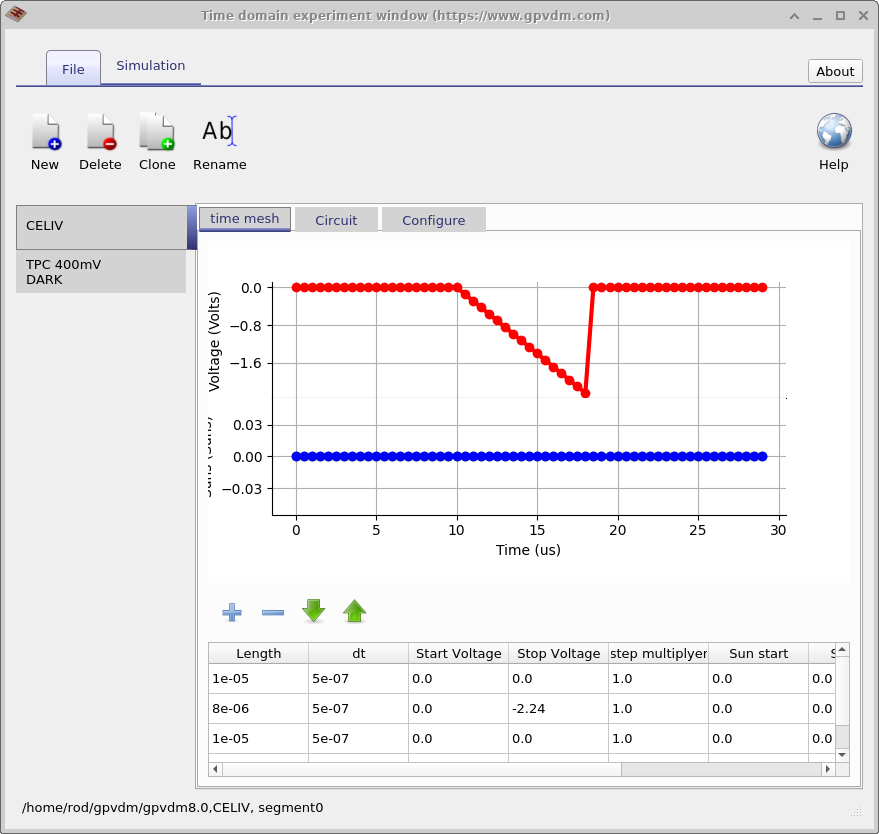
\includegraphics[width=0.5\textwidth,height=0.4\textwidth]{./images/time_domain_editor.png}

&
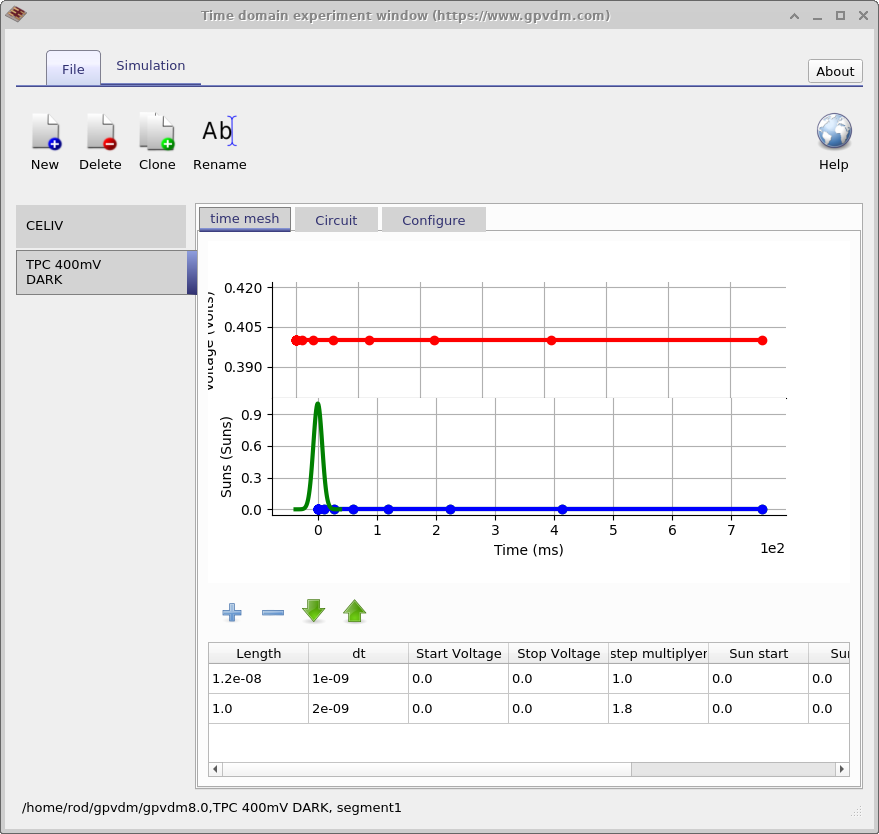
\includegraphics[width=0.5\textwidth,height=0.4\textwidth]{./images/time_domain_editor2.png}

\\

\end{tabular}
\caption{The time domain editor showing the user editing the duration of light/voltage pulses.}
\label{fig:timedomaineditor}
\end{figure}

Figure \ref{fig:timedomaineditor2} shows different tabs in of the time domain editor. The image on the left shows the circuit diagram used to model the CELIV experiment. The diode on the left represents the drift diffusion simulation while the other components represent various parasitic components.  After the diode from the left next comes a capacitor used to model the charge on the plates of the device, then a shunt resistance and then the series resistance.  The final resistor on the right represents the external resistance of the measuring equipment, this is by default set to zero but worth checking. The drop down menu on the top left of the image above the circuit diagram says \emph{load type}, this can change the load the circuit from what is shown in the picture, to a perfect diode where no parasitic components are shown to a device at open circuit which would be used to simulate Transient Photo Voltage measurements.  The right hand figure shows the configuration options of the time domain window. Again notice the \emph{Output verbosity to disk} option as described in the previous section, you will see this again and again in OghmaNano.

\newpage
\begin{figure}
\centering
\begin{tabular}{ c c }

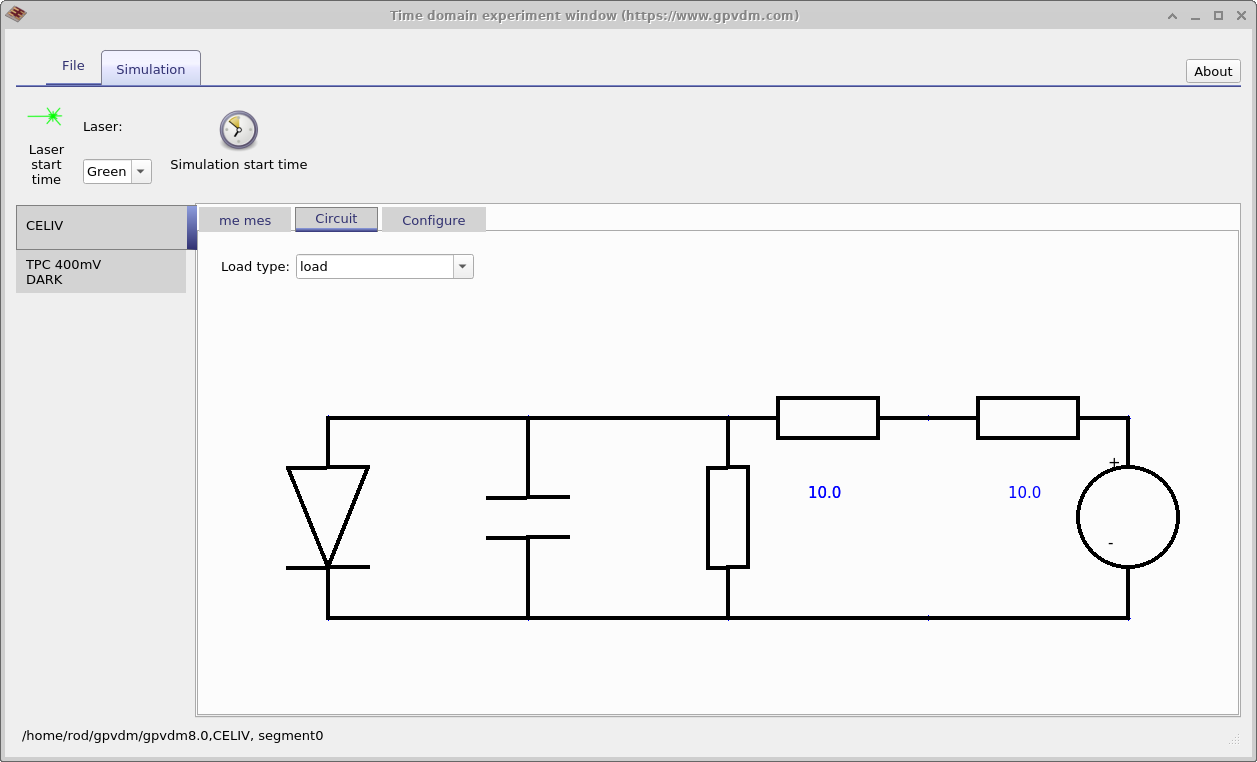
\includegraphics[width=0.5\textwidth,height=0.4\textwidth]{./images/time_domain_editor1.png}

&
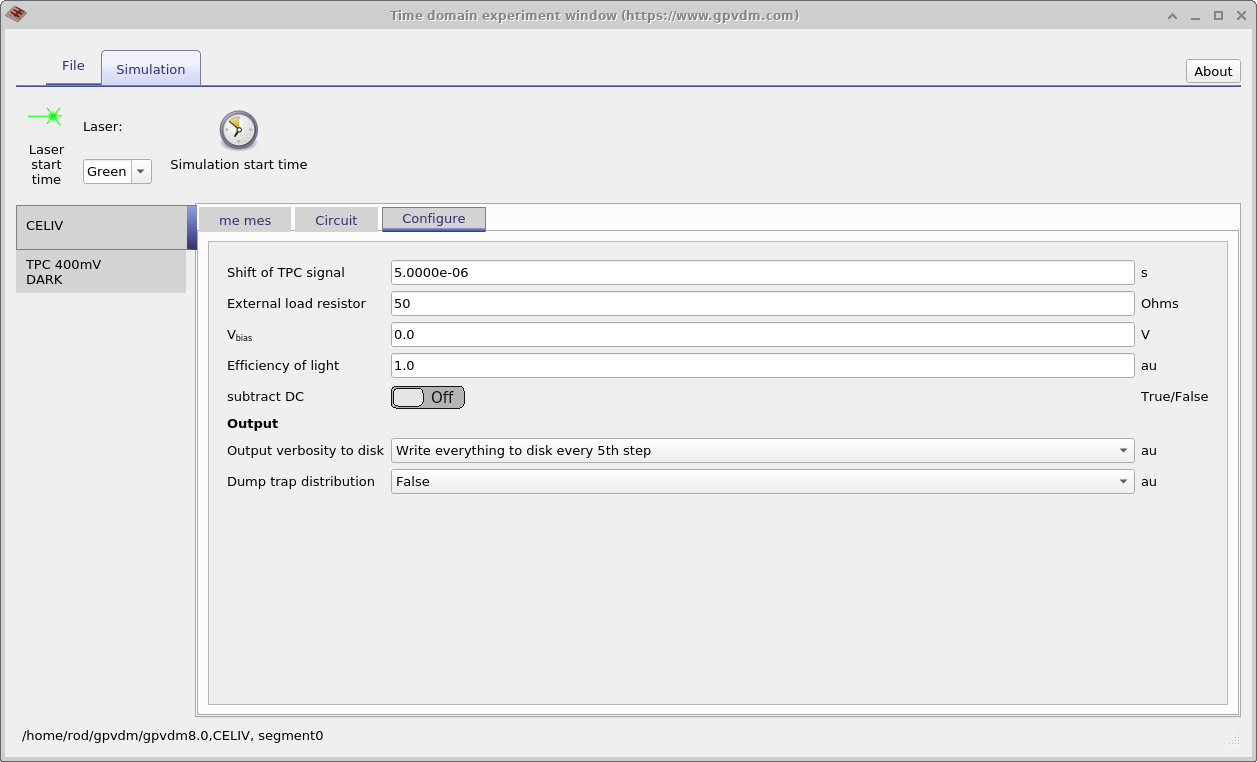
\includegraphics[width=0.5\textwidth,height=0.4\textwidth]{./images/time_domain_editor4.png}

\end{tabular}
\caption{Configuring the time domain editor: Left the circuit diagram used by the time domain window and right simulation options.}
\label{fig:timedomaineditor2}
\end{figure}

\vspace*{\fill}
